% !TEX program = pdflatex
\documentclass[aspectratio=169,xcolor=dvipsnames]{beamer}
\usetheme{SimplePlus}

\usepackage{graphicx,booktabs,mathtools,xspace,tikz}
\usetikzlibrary{arrows.meta,positioning,calc,fit}
\usepackage[natbib=true,backend=biber,style=authoryear,maxbibnames=99]{biblatex}
\setbeamertemplate{bibliography item}[article]
\renewcommand*{\bibfont}{\footnotesize}
\addbibresource{predicates.bib}
% Selected notation from predicates.tex / newcommands.tex.
\newcommand{\set}[1]{\{#1\}}
\newcommand{\tuple}[1]{\langle#1\rangle}
\newcommand{\Key}{{\sf K}}
\newcommand{\Val}{{\sf V}}
\newcommand{\Predicate}{{\sf P}}
\newcommand{\predread}{{\sf PR}}
\newcommand{\itemwrite}{{\sf W}}
\newcommand{\match}{\Delta}
\newcommand{\T}{\mathcal{T}}
\newcommand{\History}{\mathcal{H}}
\newcommand{\G}{\mathcal{G}}
\newcommand{\VIS}{\mathsf{VIS}}
\newcommand{\AR}{\mathsf{AR}}
\newcommand{\SO}{\mathsf{SO}}
\newcommand{\WR}{\mathsf{WR}}
\newcommand{\WW}{\mathsf{WW}}
\newcommand{\RW}{\mathsf{RW}}
\newcommand{\PredWR}{\mathsf{PredWR}}
\newcommand{\PredRW}{\mathsf{PredRW}}
\newcommand{\PredRWCAV}{\mathsf{PredRW}^{+}}
\newcommand{\PredRWarXiv}{\mathsf{PredRW}^{-}}
\newcommand{\si}{\mathsf{SI}}
\newcommand{\ser}{\mathsf{SER}}
\newcommand{\rel}[1]{\xrightarrow{#1}}
\newcommand{\ncite}[1]{\textcolor{black!55}{\scriptsize\cite{#1}}}


\title[Predicates and Consistency]{Specifying and Analyzing Transactional Consistency Models with Predicates}
\author{\textcolor{MidnightBlue}{\textbf{Hengfeng Wei}} \and Si Liu \and Yuxing Chen}
\institute{Hunan University \and Texas A\&M University \and Renmin University of China}
\date{September 4, 2026}

\newcommand{\accentred}[1]{\textcolor{BrickRed}{#1}}
\newcommand{\darkblue}[1]{\textcolor{MidnightBlue}{#1}}

\begin{document}

\begin{frame}
  \titlepage
  \vfill
  \centering\small\textcolor{black!55}{A semantic and graph-theoretic foundation for predicate operations}
\end{frame}

% item-predicate.tex

\begin{frame}{Item Operations vs. Predicate Operations}
  \begin{columns}[c,onlytextwidth]
    \column{0.30\textwidth}
      \begin{center}
        \fig{.75}{tikz/item-operations.pdf}\\[1.0em]
        \blue{point access}\\[0.2em]
        {returns one value}
      \end{center}
    \column{0.30\textwidth}
      \begin{center}
        \large\textbf{Employee}\\[.45em]
        \renewcommand{\arraystretch}{1.25}
        \begin{tabular}{cc}
          \toprule
          EID & Salary \\
          \midrule
          0 & 80 \\
          1 & 100 \\
          {2} & {60} \\
          {3} & {40} \\
          \bottomrule
        \end{tabular}
      \end{center}
    \column{0.40\textwidth}
    \begin{center}
      \fig{.70}{tikz/predicate-read.pdf}\\[1.0em]
      \red{condition-based access}\\[0.2em]
      {returns a set $M$ of {\bf matched} values}
    \end{center}
  \end{columns}
\end{frame}
% review-wo-predicates.tex

\begin{frame}{Review}
  \begin{center}
    {\LARGE
      What we know about transactional consistency models \\[1em]
      \red{without predicates}}
  \end{center}
\end{frame}

\begin{frame}{Review: Intuitive or Operational Specs}
  \begin{columns}[c,onlytextwidth]
    \column{0.45\textwidth}
      \begin{center}
        \ncite{Notions:CACM1976} \\[1em]
        \fig{.60}{figs/notions-cacm1976.png}\\[0.6em]
        \blue{\Large\bfseries SER}\\[.1em]
        {serial execution}
      \end{center}
    \column{0.45\textwidth}
      \begin{center}
        \ncite{CritiqueSQL:SIGMOD1995} \\[1em]
        \fig{.60}{figs/critique-sigmod1995.png}\\[.35em]
        \fig{.42}{figs/si-sigmod1995.png}\\[0.6em]
        \blue{\Large\bfseries SI}\\[.1em]
        {snapshot + write-conflict control}
      \end{center}
  \end{columns}
\end{frame}

\begin{frame}{Review: Axiomatic Specs}
  \begin{center}
    \ncite{Cerone:CONCUR2015} \\[1em]
    \fig{0.45}{figs/framework-concur2015.png}\\[.5em]
    \blue{$(\VIS, \AR)$}
  \end{center}

  \begin{columns}[c,onlytextwidth]
    \column{0.50\textwidth}
      \begin{center}
        \ncite{ClientCentric:PODC2017} \\[1em]
        \fig{0.90}{figs/clientcentric-podc2017.png}\\[.5em]
        \blue{Client-Centric Views}
      \end{center}
    \column{0.50\textwidth}
      \begin{center}
        \ncite{Complexity:OOPSLA2019} \\[1em]
        \fig{0.90}{figs/complexity-oopsla2019.png}\\[.5em]
        \blue{Checking Complexity}
      \end{center}
  \end{columns}
\end{frame}

\begin{frame}{Review: Dependency Graphs}
  \begin{columns}[c,onlytextwidth]
    \column{0.40\textwidth}
      \begin{center}
        \ncite{Notions:CACM1976} \\[.5em]
        \fig{.40}{figs/notions-cacm1976.png}\\[1em]
        \ncite{CC:STOC1976} \\[.5em]
        \fig{.70}{figs/cc-stoc1976.png}\\[1em]
        \ncite{Adya:PhDThesis1999} \\[.5em]
        \fig{.70}{figs/adya-phdthesis1999.png}
      \end{center}
    \column{0.55\textwidth}
    \begin{center}
    \end{center}
  \end{columns}
\end{frame}

\begin{frame}{Review: SER Characterization Theorem}
  \begin{columns}[c,onlytextwidth]
    \column{0.34\textwidth}
    \begin{center}
      \fig{.87}{figs/notions-cacm1976.png}\\[.6em]
      \fig{.87}{figs/cc-stoc1976.png}
    \end{center}

    \column{0.59\textwidth}
    \begin{center}
      \begin{theorem}
        An item-operation history is serializable iff its dependency graph is
        internally consistent and acyclic.
      \end{theorem}
    \end{center}
  \end{columns}
  \vfill\hfill\ncite{CC:Bernstein1987,Adya:PhDThesis1999}
\end{frame}

\begin{frame}{Review: SI Characterization Theorem}
  \begin{columns}[c,onlytextwidth]
    \column{0.36\textwidth}
    \begin{center}
      \fig{.80}{figs/si-sigmod1995.png}
    \end{center}

    \column{0.57\textwidth}
    \begin{center}
      \begin{theorem}
        An item-operation history satisfies SI iff its dependency graph is
        internally consistent and every cycle has two adjacent $\RW$ edges.
      \end{theorem}
    \end{center}
  \end{columns}
  \vfill
  \begin{center}
    \red{This exact correspondence is the baseline that predicates must recover.}
  \end{center}
  \vfill\hfill\ncite{AnalysingSI:JACM2018}
\end{frame}

\begin{frame}{Review: Downstream Tasks}
  \begin{center}
    \renewcommand{\arraystretch}{1.45}
    \begin{tabular}{@{}p{.30\textwidth}p{.57\textwidth}@{}}
      \toprule
      \textbf{Task} & \textbf{Representative work} \\
      \midrule
      Black-box checking & Elle, COBRA, PolySI, VeriStrong \\
      CC protocol verification & execution-based verification \\
      Robustness & robustness against weaker consistency \\
      \bottomrule
    \end{tabular}
  \end{center}
  \vfill
  \begin{center}
    \large\red{All depend on a faithful link between observed histories and consistency.}
  \end{center}
  \vfill\hfill\ncite{Elle:VLDB2020,Cobra:OSDI2020,PolySI:VLDB2023,VeriStrong:VLDB2026,RobustRA:CONCUR2016}
\end{frame}

\begin{frame}{Review (Summary)}
  \begin{center}
    \vspace{.6em}
    {\LARGE What we know about transactional consistency models}\\[.35em]
    {\LARGE\red{without predicates}}
  \end{center}
  \vfill
  \begin{center}
    \fig{.58}{tikz/item-consistency-review.pdf}
  \end{center}
\end{frame}
\begin{frame}{Review: Downstream Tasks}
  \centering
  \renewcommand{\arraystretch}{1.45}
  \begin{tabular}{@{}p{.30\textwidth}p{.57\textwidth}@{}}
    \toprule
    \textbf{Task} & \textbf{Representative work} \\
    \midrule
    Black-box checking & Elle, COBRA, PolySI, VeriStrong \\
    CC protocol verification & execution-based verification \\
    Robustness & robustness against weaker consistency \\
    \bottomrule
  \end{tabular}\vfill
  \large\red{All depend on a faithful link between observed histories and consistency.}
  \vfill\hfill\ncite{Elle:VLDB2020,Cobra:OSDI2020,PolySI:VLDB2023,VeriStrong:VLDB2026,RobustRA:CONCUR2016}
\end{frame}

\begin{frame}{Review}
  \centering\vspace{.6em}
  {\LARGE What we know about transactional consistency models}\\[.35em]
  {\LARGE\red{with predicates}}\vfill
  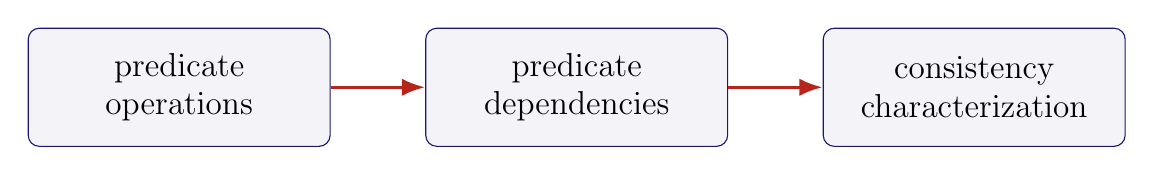
\begin{tikzpicture}[>=Latex,font=\large,
      box/.style={draw=MidnightBlue,rounded corners=4pt,fill=MidnightBlue!5,
        text width=36mm,minimum height=15mm,align=center}]
    \node[box] (p) {predicate\\operations};
    \node[box,right=12mm of p] (d) {predicate\\dependencies};
    \node[box,right=12mm of d] (c) {consistency\\characterization};
    \draw[-Latex,very thick,BrickRed] (p) -- (d);
    \draw[-Latex,very thick,BrickRed] (d) -- (c);
  \end{tikzpicture}\vfill
  \large\blue{The question now includes which items a query did not return.}
\end{frame}

\begin{frame}{Review: Intuitive or Operational Specs}
  \begin{columns}[c,onlytextwidth]
    \begin{column}{.46\textwidth}\centering
      \fig{.70}{figs/notions-cacm1976.png}\\[.6em]
      {\Large\bfseries SER}\\[.35em]\blue{serial execution}
    \end{column}
    \begin{column}{.46\textwidth}\centering
      \fig{.63}{figs/critique-sigmod1995.png}\\[.35em]
      \fig{.43}{figs/si-sigmod1995.png}\\[.25em]
      {\Large\bfseries SI}\quad \red{snapshot + write-conflict control}
    \end{column}
  \end{columns}\vfill
  \centering\large Predicate semantics is not supplied by these item-level specifications.
  \vfill\hfill\ncite{Notions:CACM1976,CritiqueSQL:SIGMOD1995}
\end{frame}

\begin{frame}{Review: Axiomatic Specs}
  \begin{columns}[c,onlytextwidth]
    \begin{column}{.44\textwidth}\centering
      \fig{.93}{figs/complexity-cav2025.png}\\[.7em]
      \blue{checking-oriented consistency conditions}
    \end{column}
    \begin{column}{.44\textwidth}\centering
      \fig{.93}{figs/specs-cav2025.png}\\[.7em]
      \blue{axiomatic specification grammar}
    \end{column}
  \end{columns}\vfill
  \centering\large\red{The challenge: make the specification explain matching and omitted items.}
  \vfill\hfill\ncite{ComplexityMIL:CAV2025}
\end{frame}

\begin{frame}{Review: Dependency Graphs}
  \begin{columns}[c,onlytextwidth]
    \begin{column}{.42\textwidth}\centering
      \fig{.87}{figs/adya-phdthesis1999.png}
    \end{column}
    \begin{column}{.51\textwidth}\centering
      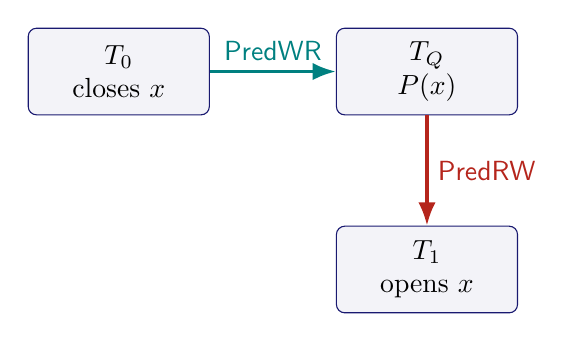
\begin{tikzpicture}[>=Latex,font=\normalsize,
          tx/.style={draw=MidnightBlue,rounded corners=3pt,fill=MidnightBlue!5,
            minimum width=23mm,minimum height=11mm,align=center}]
        \node[tx] (w) {$T_0$\\closes $x$};
        \node[tx,right=16mm of w] (q) {$T_Q$\\$P(x)$};
        \node[tx,below=14mm of q] (u) {$T_1$\\opens $x$};
        \draw[-Latex,very thick,teal] (w) -- node[above] {$\PredWR$} (q);
        \draw[-Latex,very thick,BrickRed] (q) -- node[right] {$\PredRW$} (u);
      \end{tikzpicture}\\[.7em]
      \small A predicate read depends on a witness and on later result-changing writers.
    \end{column}
  \end{columns}\vfill\hfill\ncite{Adya:PhDThesis1999}
\end{frame}

\begin{frame}{Review: Dependency Graphs}
  \begin{columns}[c,onlytextwidth]
    \begin{column}{.29\textwidth}\centering
      \fig{.92}{figs/adya-icde2000.png}\\[.5em]
      \small generalized isolation
    \end{column}
    \begin{column}{.29\textwidth}\centering
      \fig{.92}{figs/vbox-arxiv2025.png}\\[.5em]
      \small earliest result change
    \end{column}
    \begin{column}{.29\textwidth}\centering
      \fig{.92}{figs/complexity-cav2025.png}\\[.5em]
      \small all later writers
    \end{column}
  \end{columns}\vfill
  \centering\Large $\PredRWarXiv \subseteq \PredRW \subseteq \PredRWCAV$\\[.5em]
  \large\red{Predicate-read and predicate-anti-dependency definitions differ.}
  \vfill\hfill\ncite{Adya:ICDE2000,Vbox:arXiv2025,ComplexityMIL:CAV2025}
\end{frame}

\begin{frame}{Review: SER Characterization}
  \begin{columns}[c,onlytextwidth]
    \begin{column}{.38\textwidth}\centering
      \fig{.90}{figs/proof-phdthesis1999.png}
    \end{column}
    \begin{column}{.54\textwidth}\centering
      \large Item-level serializability has a well-established graph proof.\\[.9em]
      \red{Predicate extensions use different edges, but lack a single rigorous semantic proof bridge.}
    \end{column}
  \end{columns}\vfill
  \hfill\ncite{CC:Bernstein1987,TP:Gray1993,Adya:PhDThesis1999,Adya:ICDE2000,MakingSISER:TODS2005,Emme:EuroSys2024,Emme:TOCS2026,Vbox:arXiv2025}
\end{frame}

\begin{frame}{Review: SI Characterization}
  \begin{columns}[c,onlytextwidth]
    \begin{column}{.39\textwidth}\centering
      \fig{.88}{figs/adya-phdthesis1999.png}
    \end{column}
    \begin{column}{.54\textwidth}\centering
      \large Item-level SI requires two adjacent anti-dependencies in every cycle.\\[.9em]
      \red{Which predicate edges preserve this exact characterization?}
    \end{column}
  \end{columns}\vfill\hfill\ncite{Adya:PhDThesis1999,AnalysingSI:JACM2018}
\end{frame}

% problem.tex

\begin{frame}{What the Missing Bridge Must Deliver}
  \begin{columns}[T,onlytextwidth]
    \column{.47\textwidth}
      \begin{block}{Semantic side}
        A predicate observation is explained by the latest visible version of
        every externally observed key, including an omitted key.
      \end{block}
      \begin{block}{Graph side}
        Predicate read- and anti-dependencies must encode the explanatory
        version and every observation-changing later write.
      \end{block}
    \column{.47\textwidth}
      \begin{alertblock}{Characterization obligation}
        \centering
        $\ser{} / \si{}$ execution exists
        \quad$\Longleftrightarrow$\quad
        a graph satisfying the corresponding criterion exists.
      \end{alertblock}
      \vspace{.6em}
      \large The reverse implication is the hard one: construct a legal
      execution \emph{from} a graph without losing predicate semantics.
  \end{columns}
\end{frame}

\end{document}
